% ==== DISCRIMINATING AGAINST QCD Zy PRODUCTION SECTION ====

The biggest challenge in this analysis is managing the dominant background,
\QCDZy production. The background estimates given in Table
\ref{tab:vzy-bg-yields} demonstrate the scale of this challenge.
Like the signal process, this background has a real Z
boson and photon. The difference is the origin of the jets, here not from a
boson decay but from \ac{QCD} production mechanisms, as shown in Figure
\ref{fig:vbs-qcdfeynman}.
%
Identifying and exploiting the differences in jet kinematics between this
background and the signal is therefore key to maximising the sensitivity of the
measurement. This section is dedicated to discussing this problem; the word
`signal' is therefore used here to refer to \ac{EW} V\Zy production and `background'
refers solely to \QCDZy production.

%TODO give Feynman diagrams? Or reference previous Feynmans

% Talk about kinematic differences
There are a small number of kinematic distributions which exhibit a large
difference between signal and background that could be exploited effectively by
a simple cut. The dijet mass, $m_{jj}$, is an obvious example as it
peaks around the W/Z boson mass for the signal but is relatively flat for the
background.
%
For many more variables however, the differences are more subtle. There may be
a clear difference in shape between signal and background
but there is no obvious cut or set of cuts that would create a signal-rich
region. Figure \ref{fig:vzy-bdt-ewvqcd} shows some distributions with the
largest signal-background discrepancies.

% m_jj and cos_theta_CS_jj show cuttable differences

\begin{figure}[tbp]
  \begin{subfigure}{.49\textwidth}
    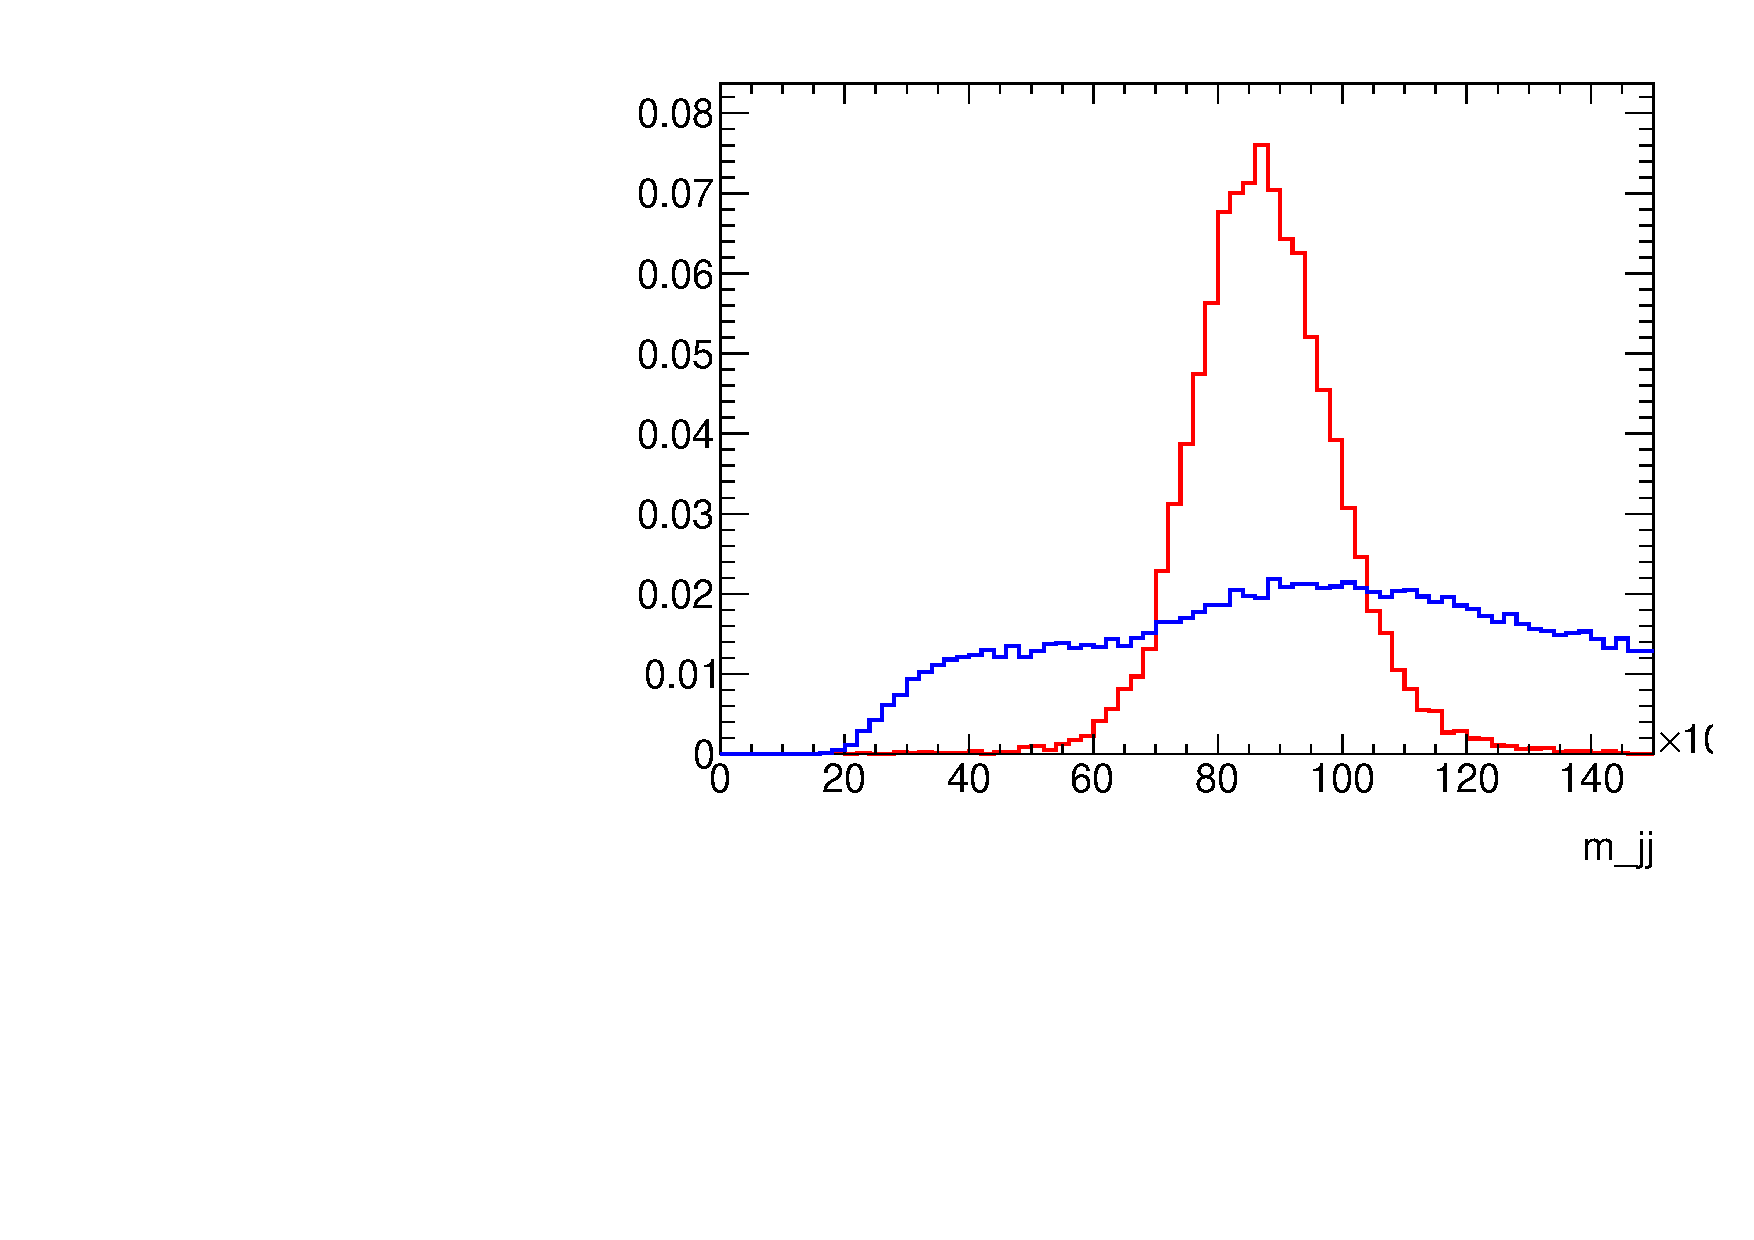
\includegraphics[width=\textwidth]{\resource{EWvQCD/m_jj.pdf}}
    \vspace{-.9cm}
    \caption{}
    \label{fig:vzy-bdt-ewvqcd-mjj}
  \end{subfigure}
  \hfill
  \begin{subfigure}{.49\textwidth}
  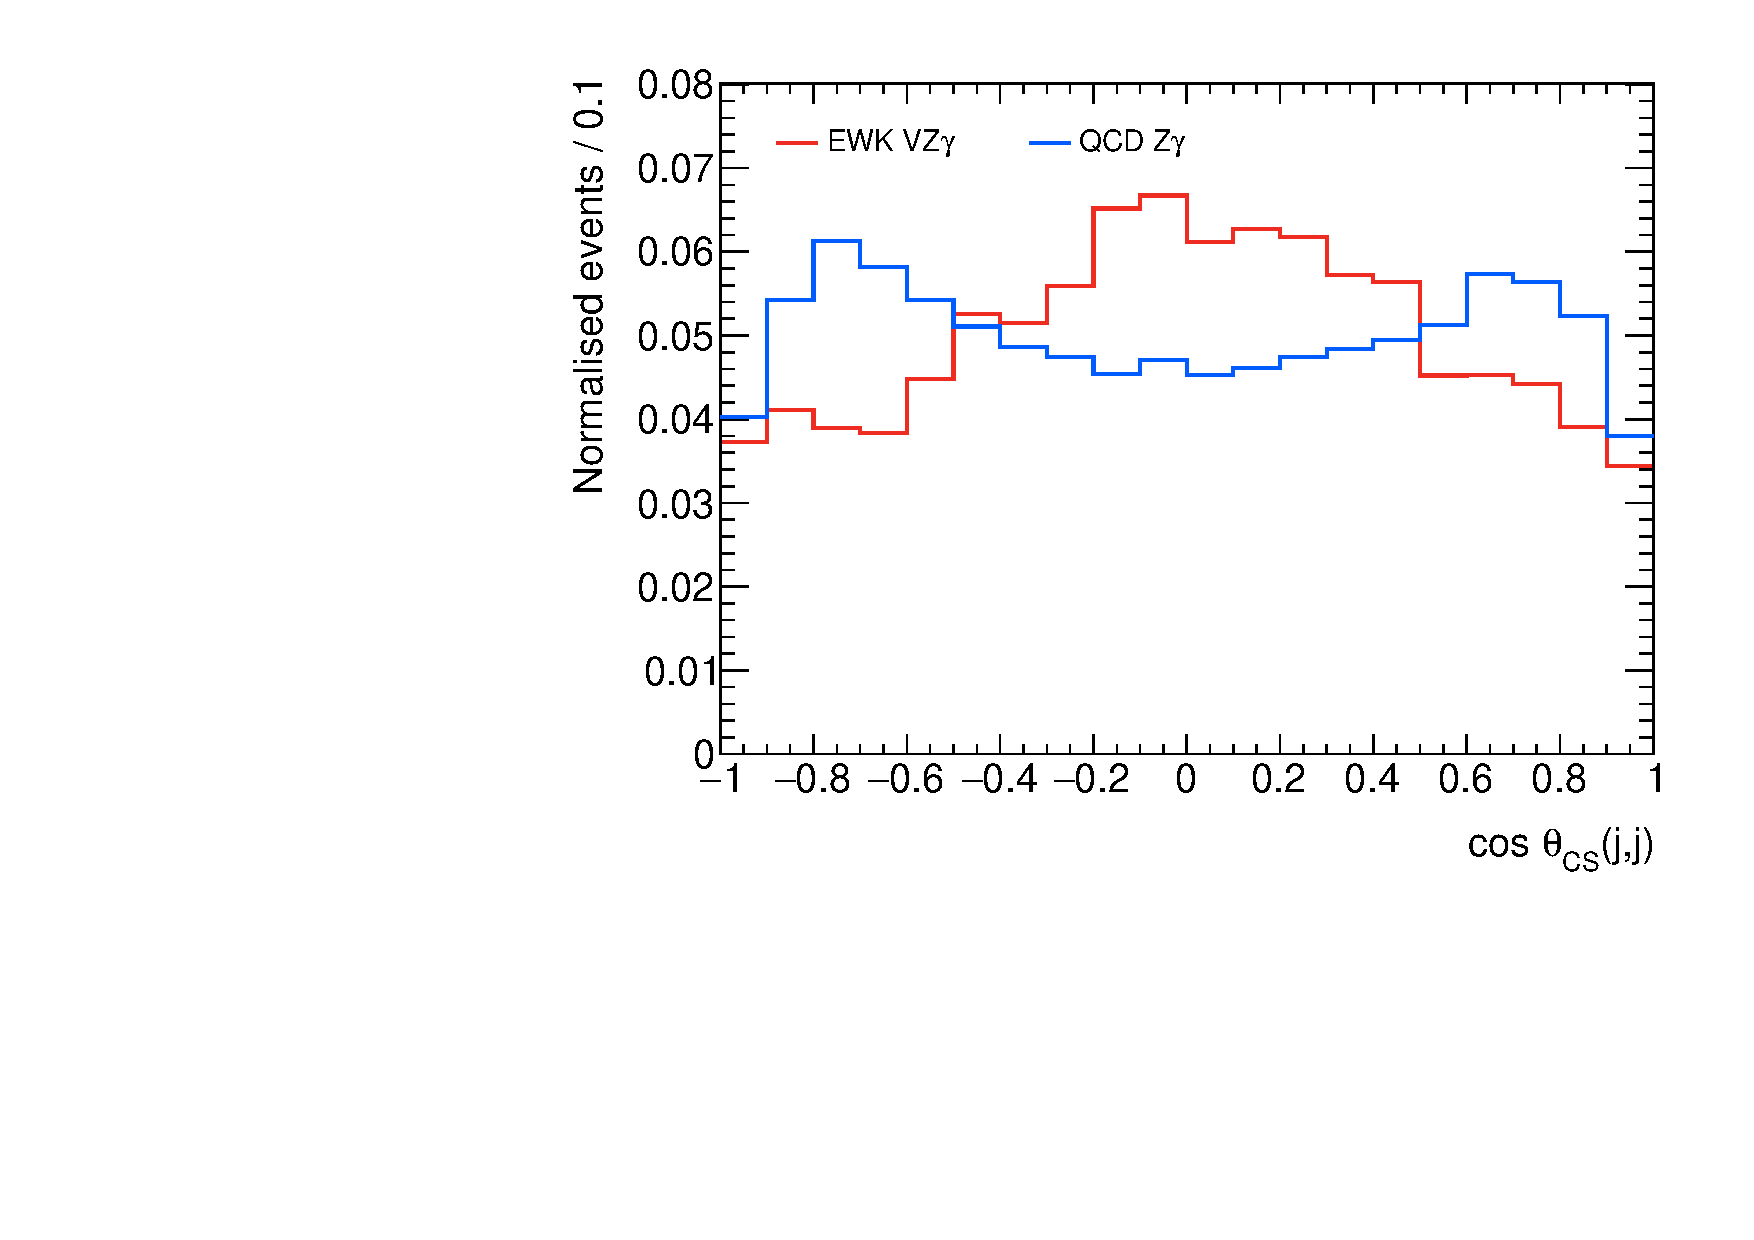
\includegraphics[width=\textwidth]{\resource{EWvQCD/cos_theta_CS_jj.pdf}}
    \vspace{-.9cm}
    \caption{}
  \end{subfigure}
  \\[.5cm]
  \begin{subfigure}{.49\textwidth}
    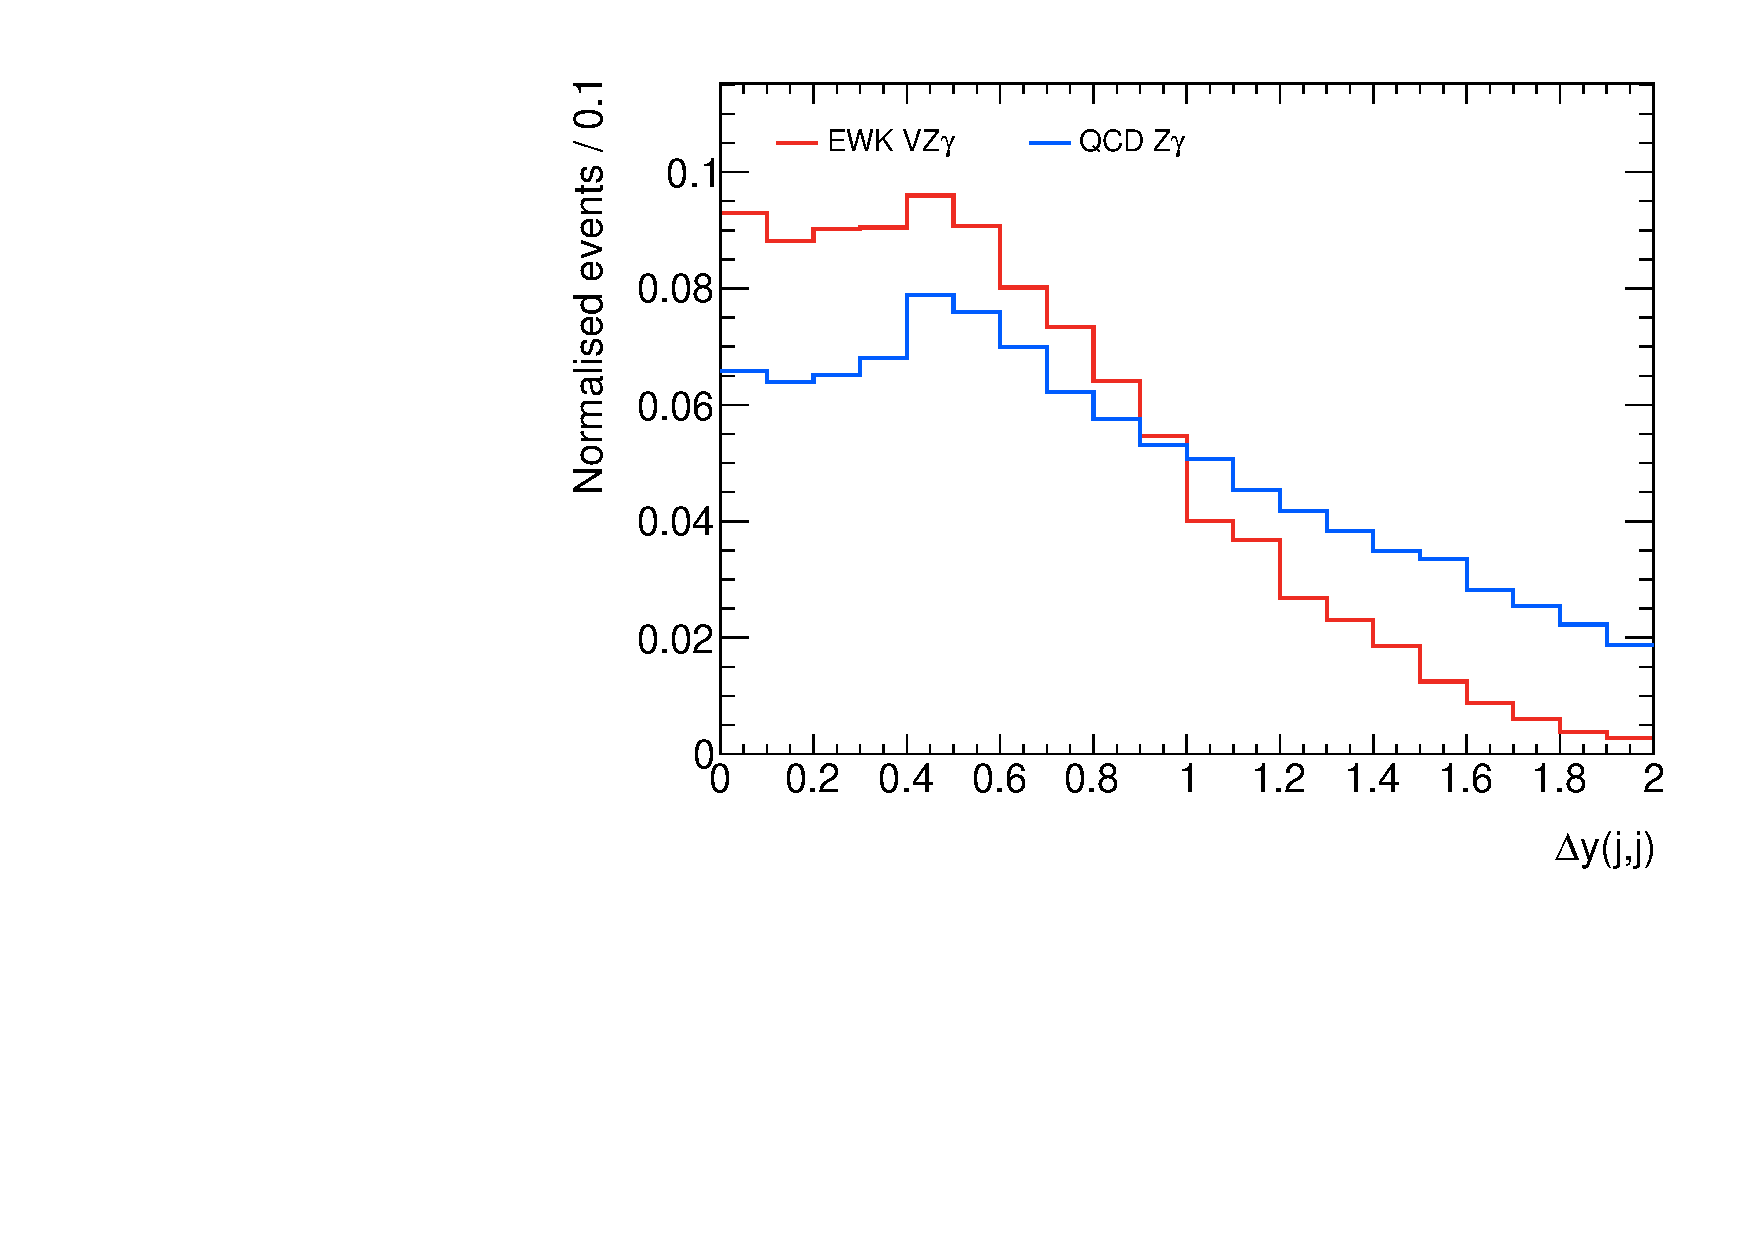
\includegraphics[width=\textwidth]{\resource{EWvQCD/Dy_j_j.pdf}}
    \vspace{-.9cm}
    \caption{}
  \end{subfigure}
  \hfill
  \begin{subfigure}{.49\textwidth}
    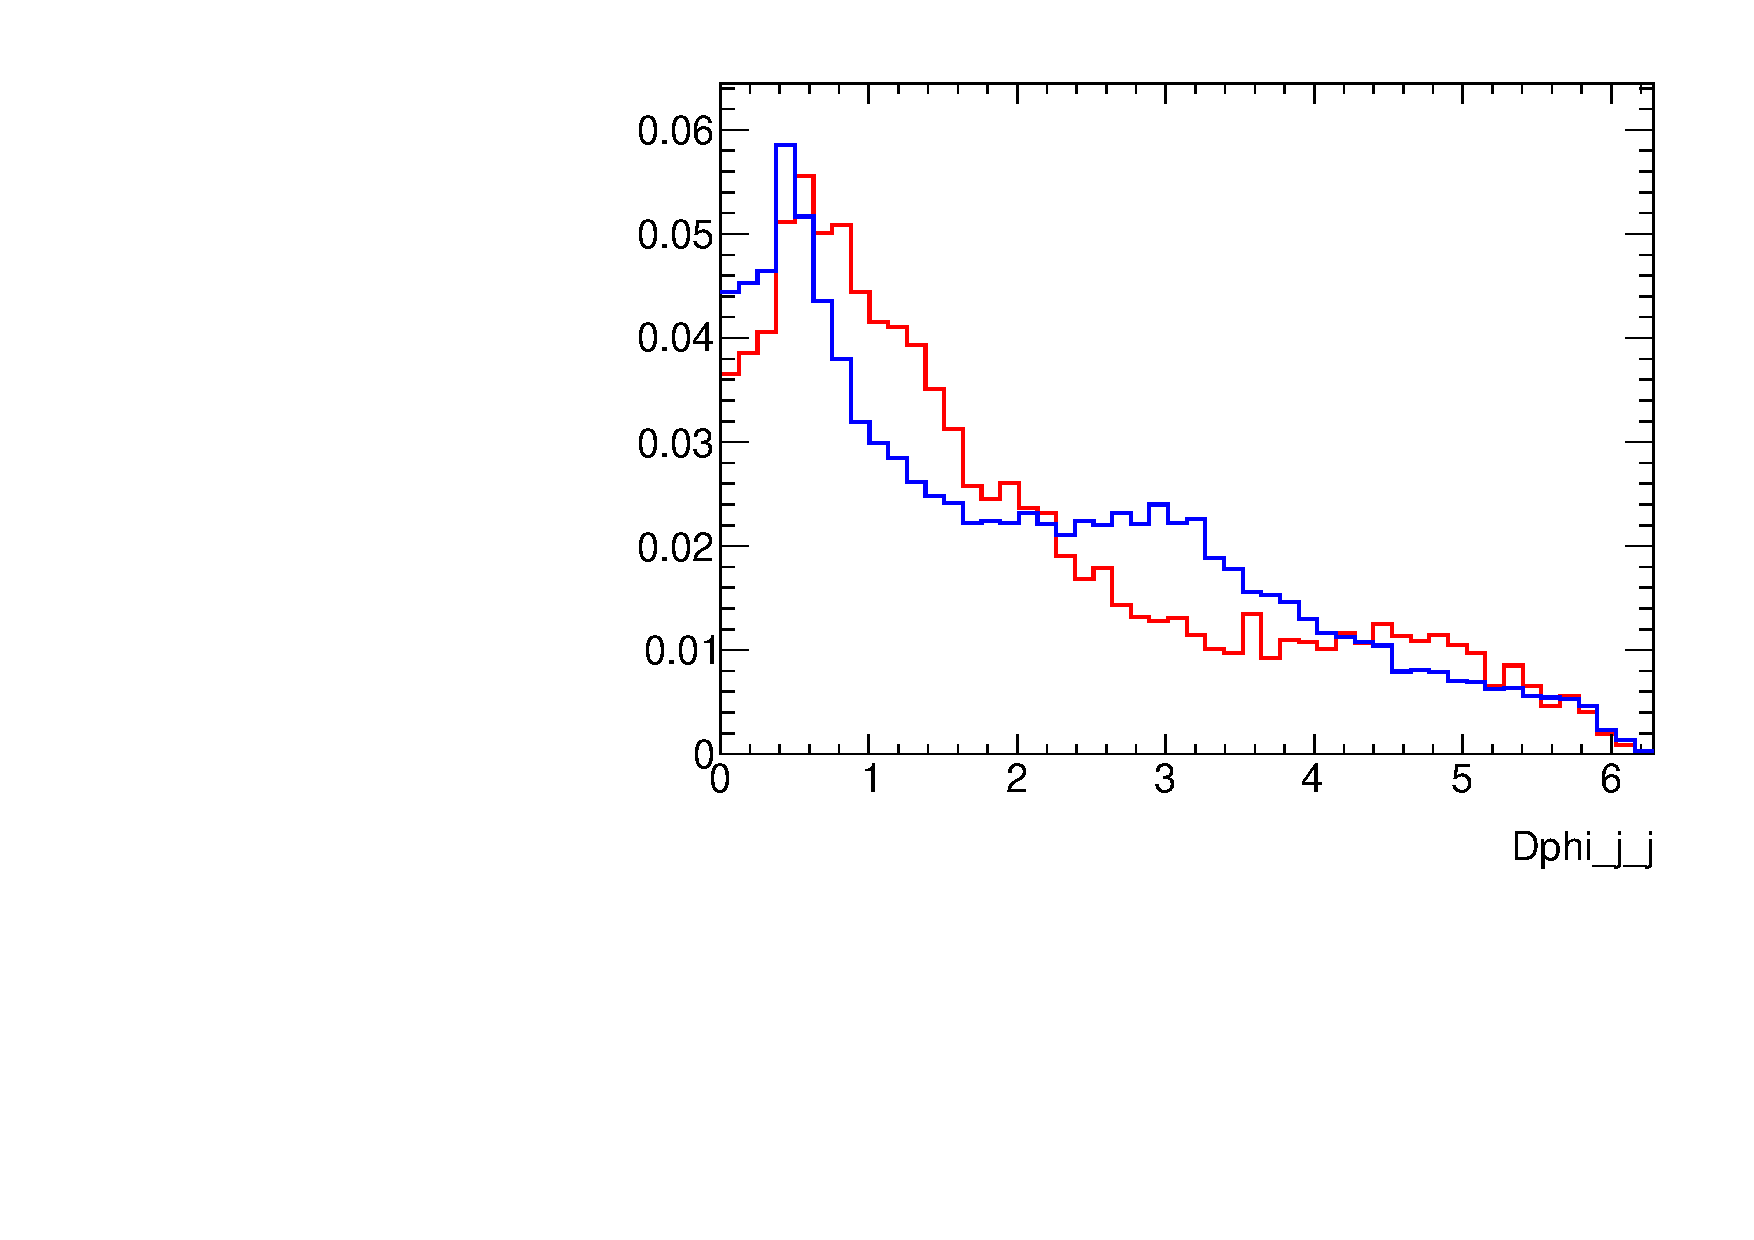
\includegraphics[width=\textwidth]{\resource{EWvQCD/Dphi_j_j.pdf}}
    \vspace{-.9cm}
    \caption{}
  \end{subfigure}
  \\[.5cm]
  \begin{subfigure}{.49\textwidth}
    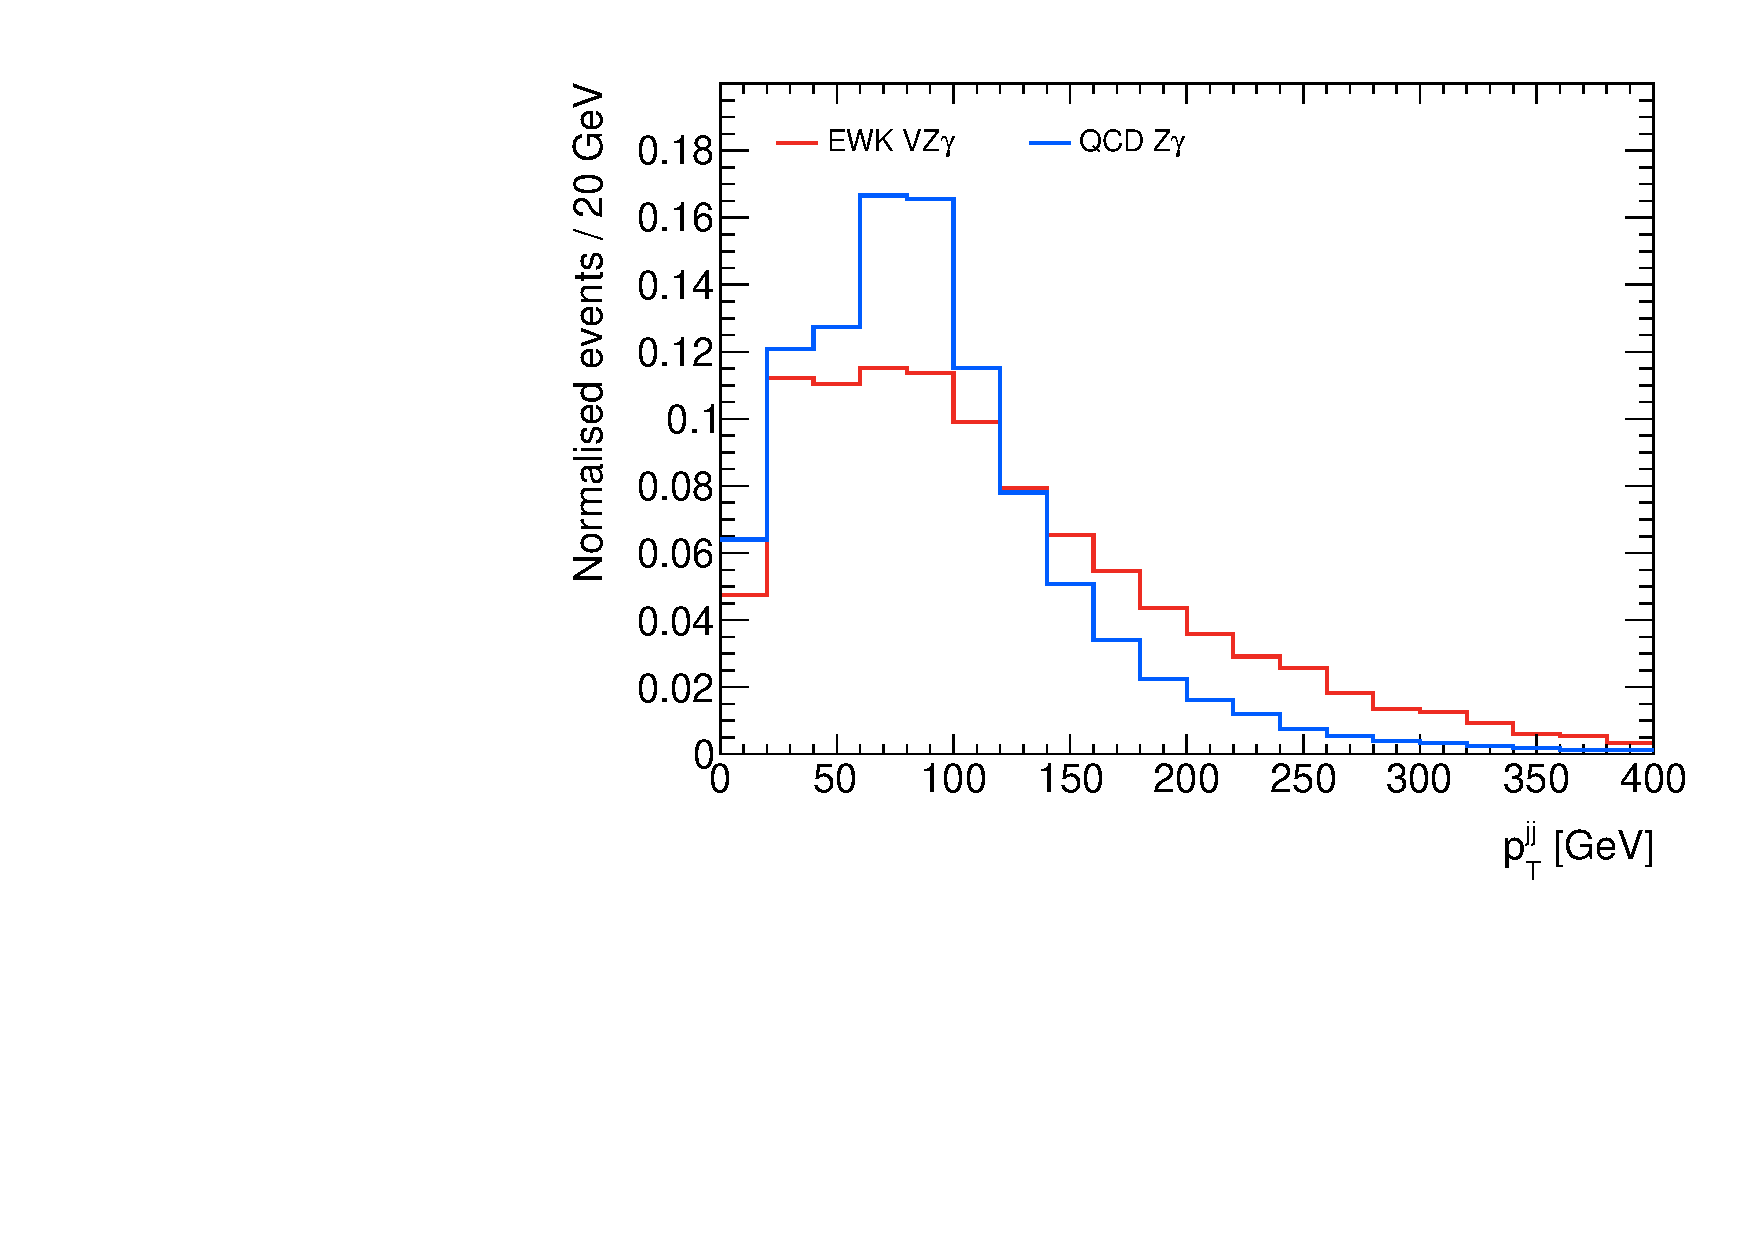
\includegraphics[width=\textwidth]{\resource{EWvQCD/pT_jj.pdf}}
    \vspace{-.9cm}
    \caption{}
  \end{subfigure}
  \hfill
  \begin{subfigure}{.49\textwidth}
    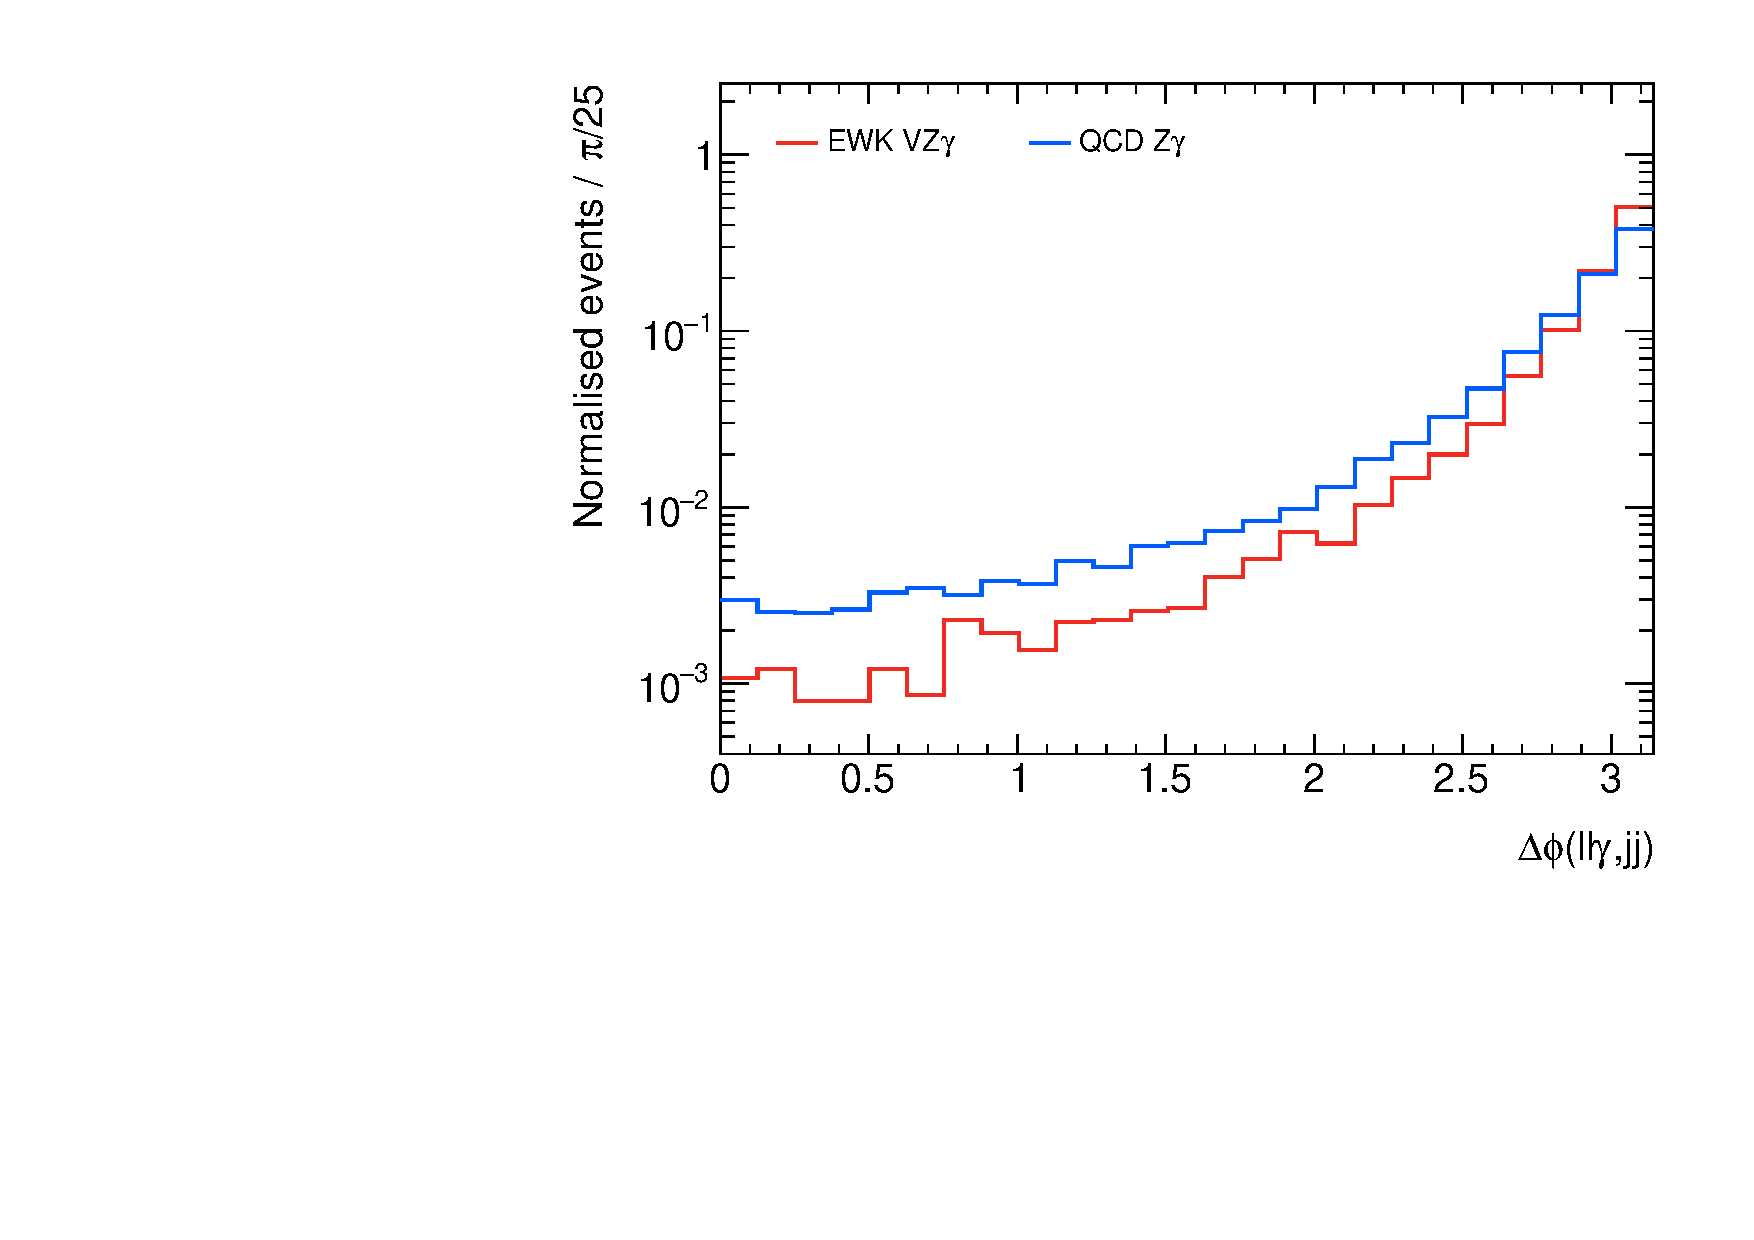
\includegraphics[width=\textwidth]{\resource{EWvQCD/Dphi_lly_jj.pdf}}
    \vspace{-.9cm}
    \caption{}
  \end{subfigure}
  %
  \caption{
    Kinematic distributions, comparing \acs{EW} V\Zy production (red) to
    \QCDZy production (blue), generated from the corresponding \ac{MC}
    samples with the analysis region selection applied. Events are normalised to
    compare the shape of distributions between the two samples. Definitions for
    the variables shown are given in Table \ref{tab:vzy-bdt-variables}.
  }
  \label{fig:vzy-bdt-ewvqcd}
\end{figure}

Creating an effective cut-based selection on these variables is relatively
ineffective; a machine-learning discriminant can be used to improve sensitivity
to the signal process.  To demonstrate this, this section explores and compares
two methods for defining a signal-sensitive phase space for the analysis: a
cut-based approach and a \ac{BDT}, a machine learning classifier introduced in
Section \ref{sec:methods-bdt}.

The dijet mass variable is excluded from selections for both of
these methods. This allows it to be used to define \acp{CR} with a low signal
purity in order to validate background estimates with comparisons to data. For
more detail on the definition and use of these \acp{CR}, see Section
\ref{sec:vzy-srcr}.

These initial investigations were performed before details of the analysis
were finalised and so have a somewhat broader phase space, detailed below.

% Section giving samples and phase-space for this study
\subsection{Phase space for preliminary studies}

The studies presented in this section use events from the \ac{EW} \VZy sample
(as defined in Section \ref{sec:vzy-selection-vzy}) as the signal and from the
\QCDZy sample as the background. All events are subject to the
preselection in Table \ref{tab:vzy-bdt-preliminaryselection}.  These cuts select
\Zy events with a looser version of the full \Zy selection presented in
Section \ref{sec:methods-selection}.  No cuts are placed on the jets at this
stage.  Isolation, identification, and overlap removal for all objects are the
same as discussed in Section \ref{sec:methods-selection}.

\begin{table}
  \centering
  \renewcommand\arraystretch{1.3}
  \caption{
    Selection for events used in background rejection studies for the \VZy
    triboson analysis. This is the same as the \Zy selection in Table
    \ref{tab:anacom-zy-selection} but with a looser photon $p_T$ cut and no
    \acs{FSR} cut.
  }
  \begin{tabular}{p{6em}l}
    \hline\hline
    \multicolumn{2}{c}{Background rejection studies preselection} \\
    \hline
    Photon & $N_\gamma \geq 1$ \\
           & $|\eta_\gamma| < 2.37$ \\
           & (excludes $1.37 < |\eta_\gamma| < 1.52$) \\
           & $p_T^\gamma > 15$ GeV \\
    \hline
    Lepton & $N_l = 2$ (OSSF)\\
           & $|\eta_e| < 2.47$ \\
           & (excludes $1.37 < |\eta_e| < 1.52$) \\
           & $|\eta_\mu| < 2.5$ \\
           & $p_T^{l,1} > 30$ GeV \\
           & $p_T^{l,2} > 20$ GeV \\
    \hline
    Boson  & $m_{ll} > 40$ GeV \\
    \hline\hline
  \end{tabular}
  \label{tab:vzy-bdt-preliminaryselection}
\end{table}

\subsection{Comparison metric}
\label{sec:vzy-bdt-significance}

A metric is needed in order to evaluate the performance of a given selection.
Since the desired selection will be one that grants the most sensitivity to the
\VZy signal, a significance of the \ac{SM}-expected signal considering a background-only
hypothesis is used. This will emulate the significance calculation used for the
final measurement, though much simplified as it deals with only a single
background and no systematic uncertainties. Whilst the significances given here
are not directly comparable to that from the full measurement, they are comparable with
each other and will indicate which selection generates more sensitivity to the
signal process.

%\newcommand\nobsi{\ensuremath{n_\text{obs}^i}\xspace}
As the $m_{jj}$ distribution is not used for selection, it is used here to
calculate significance with a binned likelihood method.
The likelihood is
constructed as described in Section \ref{sec:methods-stats-llh-simple}, and a
likelihood ratio test is used to extract the signal. Expected yields for signal
and background are taken from \ac{MC} samples.
To obtain integer values for the data yields in each bin, the significance is
calculated many times in toy \ac{MC} experiments: in each experiment the data
values are drawn at random from a Poisson distribution with a mean equal to the
sum of signal and background events in the relevant bin. Taking the mean
significance from these toys gives the values used here.

These significances are calculated for each selection tested, given as a number
of standard deviations. As no systematics are used in this simplified
performance metric, this represents statistical uncertainty only.

\subsection{Selection variables}

Building a selection to reject the \QCDZy background relies on identifying
differences in jet kinematics, and therefore placing selection requirements on
jet-based kinematic variables. A total of 22 of variables are considered, with
the full list given in Table \ref{tab:vzy-bdt-variables}.

\newcommand\ptbalance{\ensuremath{p_T^\text{balance}}\xspace}

\begin{table}[!p]
  \centering
  \renewcommand\arraystretch{1.3}
  \caption{
    Variables considered for selection to reject \QCDZy events for the
    \VZy triboson analysis.
  }
  \begin{tabular}{c|p{10cm}}
    \hline\hline
    Variable & Definition \\
    \hline
    $y_{j,1}$ &
    Rapidity of the leading jet in the event.
    \\
    $y_{j,2}$ &
    Rapidity of the sub-leading jet in the event.
    \\
    $y_{jj}$ &
    Rapidity of the $jj$ system.
    \\
    $p_T^{j,1}$ &
    Transverse momentum of the leading jet in the event.
    \\
    $p_T^{j,2}$ &
    Transverse momentum of the sub-leading jet in the event.
    \\
    $p_T^{jj}$ &
    Transverse momentum of the $jj$ system.
    \\
    \ptbalance &
    Relative difference between transverse momenta of the $jj$ and $ll\gamma$
    systems, given by Equation \ref{eqn:vzy-bdt-ptbalance}.
    \\
    $N_j$ &
    Number of jets in the event, reconstructed with a minimum $p_T$ of 25 GeV.
    \\
    $N_j^\text{gap}$ &
    Number of jets, satisfying $p_T > 25$ GeV found in the rapidity region
    between the two leading jets.
    \\
    $m_{j,1}$ &
    Mass of the leading jet in the event.
    \\
    $m_{j,2}$ &
    Mass of the sub-leading jet in the event.
    \\
    $m(ll\gamma jj)$ &
    Mass of the triboson system.
    \\
    $|\Delta y_{jj}|$ &
    Absolute rapidity difference between the two leading jets.
    \\
    $\Delta\phi_{jj}$ &
    Smallest difference between the azimuthal angles of the two leading jets.
    \\
    $\Delta R_{jj}$ &
    $\Delta R$ value between the two leading jets.
    \\
    $|\Delta y(ll\gamma, jj)|$ &
    Absolute rapidity difference between the $ll\gamma$ and $jj$ systems.
    \\
    $\Delta\phi(ll\gamma, jj)$ &
    Smallest difference between the azimuthal angles of the $ll\gamma$ and $jj$
    systems.
    \\
    $\Delta R(ll\gamma, jj)$ &
    $\Delta R$ value between the $ll\gamma$ and $jj$ systems.
    \\
    $\Delta R_\text{min}(\gamma, j)$ &
    Minimum $\Delta R$ value between any photon and jet in the event.
    \\
    $\cos{\theta^*(jj)}$ &
    Cosine of $\theta^*(jj)$, the angle of the leading jet in the dijet
    centre-of-mass frame relative to the direction of motion of the $jj$ system.
    \\
    $\cos{\theta_\text{CS}(jj)}$ &
    Cosine of $\theta_\text{CS}(jj)$, the angle between the two jets in the
    Collins-Soper frame \cite{Collins1977}. Jet charge information isn't
    available so the angle is taken relative to the leading jet.
    \\
    $\zeta(ll\gamma)$ &
    Centrality of the $ll\gamma$ system, given by Equation
    \ref{eqn:vbs-selection-centrality}.
    \\
    \hline\hline
  \end{tabular}
  \label{tab:vzy-bdt-variables}
\end{table}

The variable \ptbalance is given by the equation

\begin{equation}
  \ptbalance = \frac{ (p_T^{jj} - p_T^{ll\gamma}) }
                    { (p_T^{jj} + p_T^{ll\gamma}) }.
  \label{eqn:vzy-bdt-ptbalance}
\end{equation}

% Section describing cut-based selection optimisation
\subsection{Cut-based background rejection}
% See plots here, from old codebase
% /mnt/naf/code/VZy-prep/extract_VZy/build/signifscan_nomjj2_SR1.pdf

The task at hand is to find a set of cuts to make, on variables from Table
\ref{tab:vzy-bdt-variables}, in order to maximise sensitivity to the signal
process. Truly optimising this, finding the best value for each cut given the
values of every other cut, is a many-dimensional problem with no easy
solution. Instead an iterative approach is taken: find the best cut on each
variable individually, take the cut which gives the best improvement
in sensitivity and add it to the selection, then re-test all other cuts on the
new subset of events.

Identifying the `best' cut to make at any stage is a little subjective. For
instance, when applying the first cut, the selection that would result in the best
significance for the signal sample is likely too aggressive to allow for
multiple effective cuts afterwards. The method used is to calculate background
rejection ($1/$fraction of background events passing a cut) as a function
of signal efficiency (fraction of signal events passing a cut) for each
variable. By eye, these distributions can then be scanned to identify a possible
cut which gives large background rejection but maintains a high signal
efficiency. This allows for multiple variables to be included in the selection
before the phase space becomes too constrained.

\begin{figure}[tbhp]
  \centering
  \includegraphics[width=.48\textwidth]{\resource{integral_pT_j2_gt_fix.pdf}}
  \includegraphics[width=.48\textwidth]{\resource{rejection_pT_j2_gt_fix.pdf}}
  \caption{
    Distributions to identify a cut on $p_T^{j,2}$. Shown are fraction of events
    for each sample that are above a given threshold value in $p_T^{j,2}$ (left)
    and background rejection as a function of the signal efficiency achievable
    using the same $p_T^{j,2}$ threshold (right).
  }
  \label{fig:vzy-bdt-rejection}
\end{figure}

Figure \ref{fig:vzy-bdt-rejection} shows the background rejection against signal
efficiency for $p_T^{j,2}$, which is chosen as the first variable to cut on.
A cut of $p_T^{j,2} > 35$ GeV is chosen, with a signal efficiency of 74\%
and a background rejection factor of 2.6.

Continuing this process, the most performant selection found consisted of five
cuts, listed in Table \ref{tab:vzy-bdt-cutbased}. Using the method described in
Section \ref{sec:vzy-bdt-significance}, the significance calculated for events
passing this selection is 1.2 standard deviations.

\begin{table}[tbh]
  \centering
  \renewcommand\arraystretch{1.3}
  \caption{
    Selection derived for baseline cut-based version of the analysis. Cuts are
    applied to the \VZy signal sample and the \QCDZy background for events
    passing the preliminary selection given in Table
    \ref{tab:vzy-bdt-preliminaryselection}.
  }
  \begin{tabular}{c}
    \hline\hline
    Cut-based selection \\
    \hline
    $p_T^{j,2} > 35 GeV$ \\
    $|\Delta y_{jj}| < 1.5$ \\
    $\Delta R(ll\gamma, jj) > 3.0$ \\
    $\Delta\phi(ll\gamma, jj) > 2.8$ \\
    $\ptbalance > -0.1$ \\
    \hline\hline
  \end{tabular}
  \label{tab:vzy-bdt-cutbased}
\end{table}


% Section describing BDT optimisation
\subsection{\acs{BDT} for background rejection}

The cut-based selection provides a baseline performance against which to
evaluate a \ac{BDT}-based selection. The \ac{BDT} can take many variables as
input and determine how likely an event is to be signal or background based on
the value of those variables, having first learned how the variables are
distributed differently between signal and background events.

The first step is to train a \ac{BDT} to identify these differences between
signal and background. Once trained, the \ac{BDT} is tested on an independent
set of events to evaluate its performance and test for overtraining.
To accommodate this train-test cycle, the signal and background samples are each
split evenly into two, one half used for training and the other for testing.

Several aspects of the \ac{BDT} are tuned to improve performance: the input
variables used by the \ac{BDT}, preselection applied to events before training,
and hyperparameters of the \ac{BDT} itself. These are discussed in the sections
below.

%What to write?
% Input variable optimisation
\subsubsection{Input variable selection}
\label{sec:vzy-bdt-variables}

The benefit of the \ac{BDT} is its ability to handle many input variables and
generate a phase space sensitive to the signal. However, giving too many
variables to the \ac{BDT} creates an overly complex model and makes it prone to
overtraining. Many iterations of input variables were tested to find a set that
is sufficiently small to prevent overtraining but with enough variables to allow
the \ac{BDT} to give a good sensitivity.

For each set of variables tested, a simple overtraining check is used. For a
cut on the \ac{BDT} output resulting in a background rejection factor of 10, the
corresponding signal efficiency is compared between the training sample and the
test sample. Overtraining would result in a higher signal efficiency in the
training sample than in the test sample. A requirement that the test sample
signal efficiency is within $10\%$ of the training sample is used to mitigate
overtraining in the \ac{BDT} model.

The sensitivity attained for a \ac{BDT} trained on a particular variable set is evaluated
by calculating the significance, through the method discussed in Section
\ref{sec:vzy-bdt-significance}. To do this, a cut must first be placed on the
\ac{BDT} output. The value chosen for this cut will affect the sensitivity, so
in each instance the cut value is scanned to find the highest attainable
significance.

After using these tests to compare many combinations of variables, the most
performant set was chosen.  The final set of 16 input variables is shown in
Table \ref{tab:vzy-bdt-ranking} ranked by their `importance' as determined by
the \ac{BDT}. See Section \ref{sec:methods-bdt-importance} for a description of
how variable importance is calculated.

\begin{table}[tbh]
  \centering
  \renewcommand\arraystretch{1.2}
  \caption{
    Ranking of variables used by the \ac{BDT} to discriminate between signal and
    background for the \VZy analysis.
  }
  \begin{tabular}{lp{4cm}r}
    \hline \hline
    Rank & Variable       & Relative importance\\
    \hline
    1  & $|\Delta y_{jj}|$          & $7.46\times10^{-2}$ \\
    2  & $p_T^{j,2}$                & $7.27\times10^{-2}$ \\
    3  & $\Delta\phi_{jj}$          & $7.24\times10^{-2}$ \\
    4  & $m_{j,2}$                  & $7.06\times10^{-2}$ \\
    5  & \ptbalance                 & $7.05\times10^{-2}$ \\
    6  & $\Delta R_\text{min}(y,j)$ & $6.50\times10^{-2}$ \\
    7  & $y_{j,2}$                  & $6.32\times10^{-2}$ \\
    8  & $\Delta\phi(ll\gamma, jj)$ & $6.15\times10^{-2}$ \\
    9  & $\cos\theta_\text{CS}(jj)$ & $6.10\times10^{-2}$ \\
    10 & $p_T^{j,1}$                & $5.76\times10^{-2}$ \\
    11 & $y_{j,1}$                  & $5.70\times10^{-2}$ \\
    12 & $p_T^{jj}$                 & $5.68\times10^{-2}$ \\
    13 & $\Delta R(ll\gamma,jj)$    & $5.68\times10^{-2}$ \\
    14 & $m_{j,1}$                  & $5.60\times10^{-2}$ \\
    15 & $\log{\zeta(ll\gamma)}$    & $5.48\times10^{-2}$ \\
    16 & $y_{jj}$                   & $4.96\times10^{-2}$ \\
    \hline\hline
  \end{tabular}
  \label{tab:vzy-bdt-ranking}
\end{table}

The logarithm of the centrality, $\zeta(ll\gamma)$, is used rather than the
linear form as this found to be more effective. This was due to the binning used
by the \ac{BDT} being insensitive to the signal-rich regions, as demonstrated in
Figure \ref{fig:vzy-bdt-centrality}.

\begin{figure}[tbhp]
  \centering
  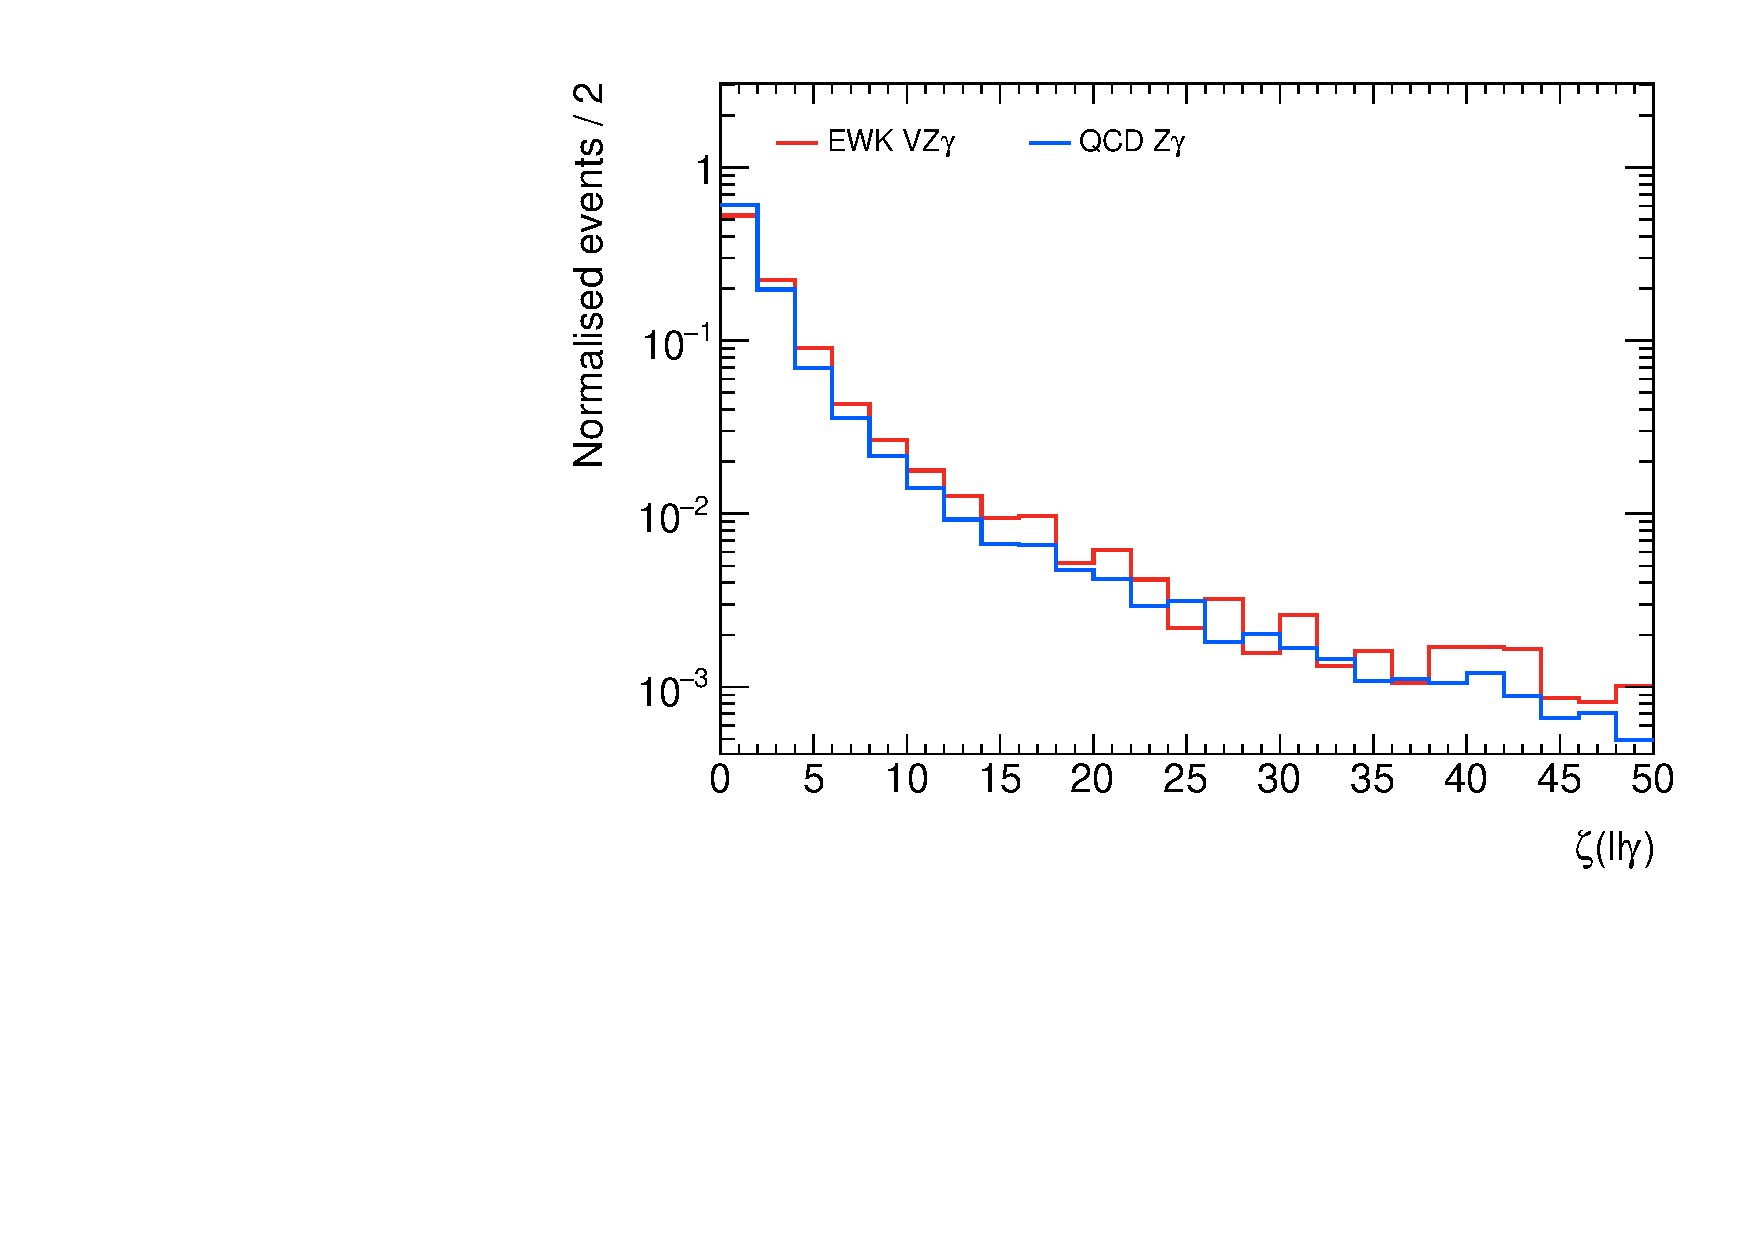
\includegraphics[width=.48\textwidth]{\resource{EWvQCD/Zy_centrality.pdf}}
  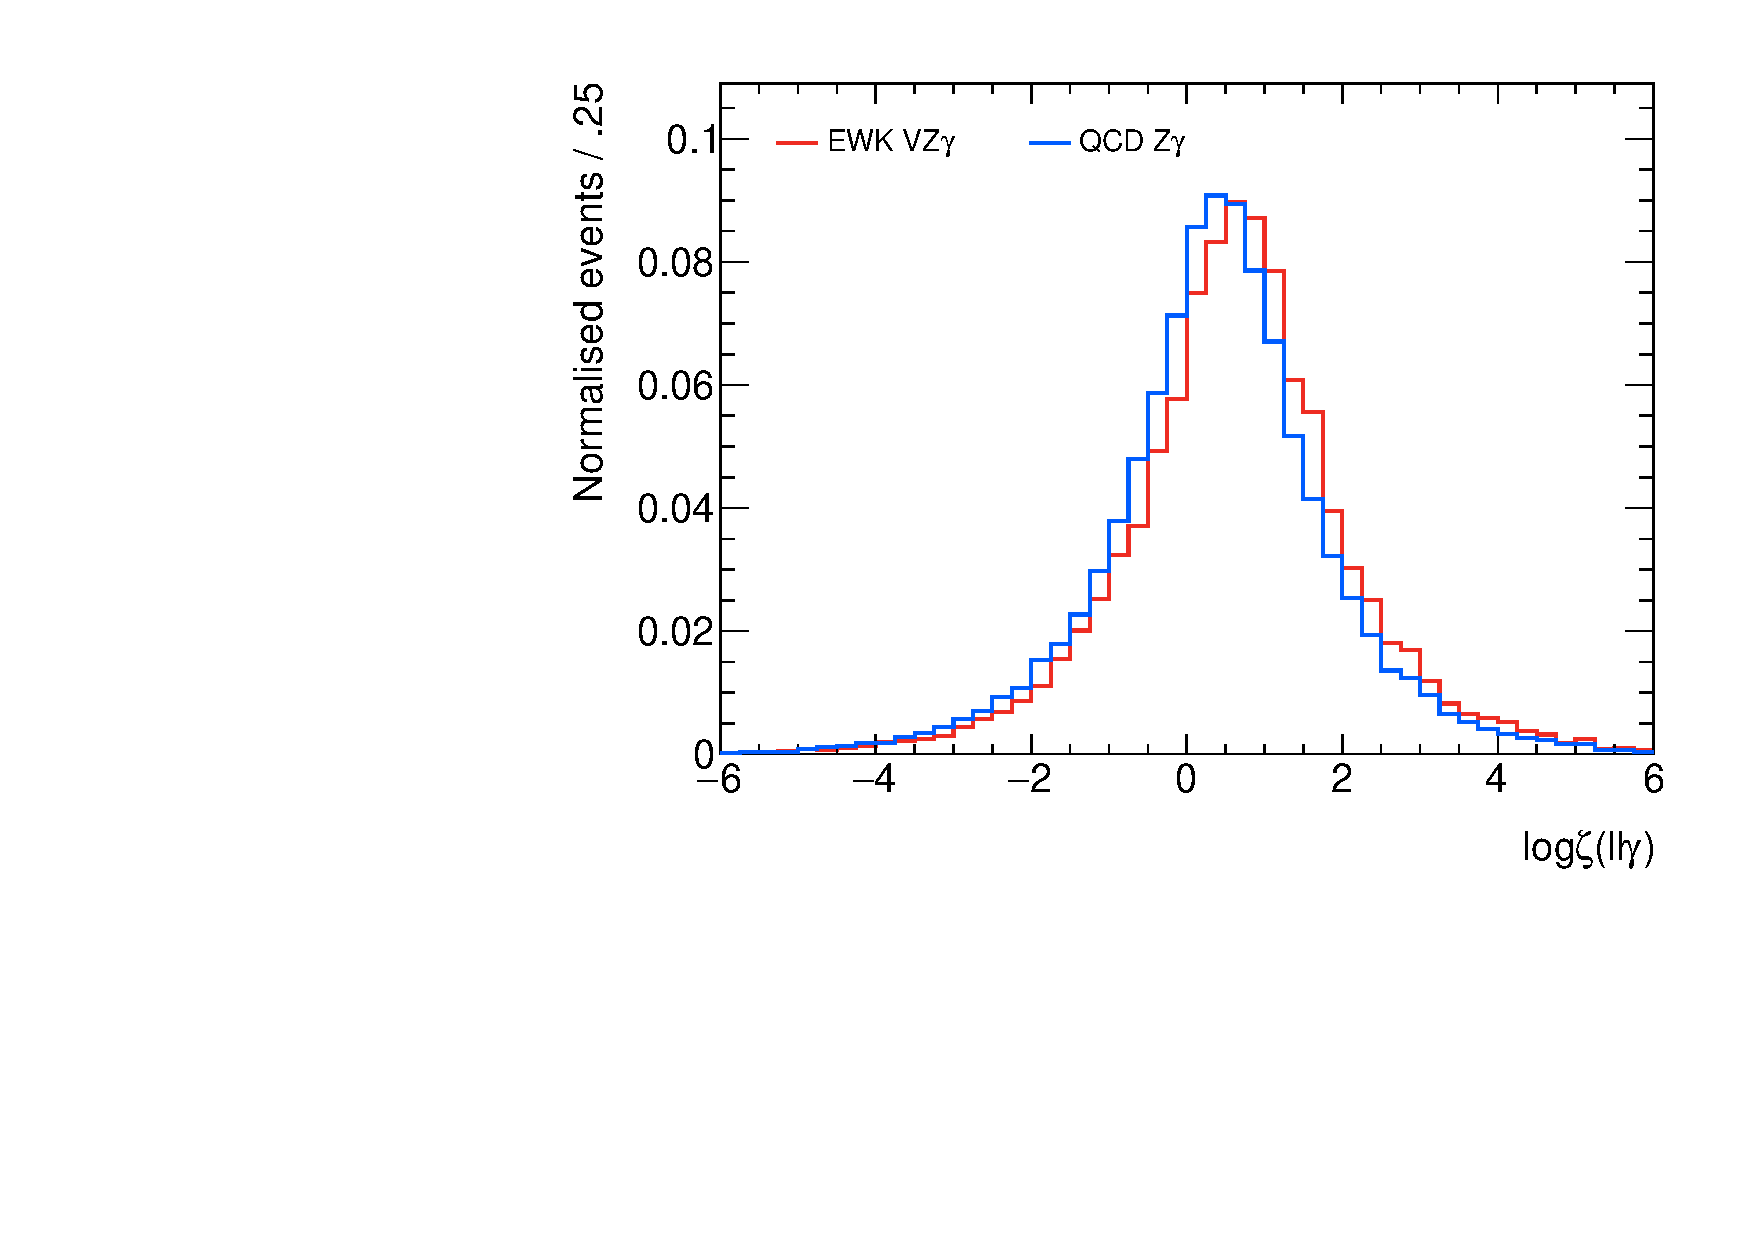
\includegraphics[width=.48\textwidth]{\resource{EWvQCD/log_Zy_centrality.pdf}}
  \caption{
    Distribution of centrality, $\zeta(ll\gamma)$, both linear (left) and
    logarithmic (right) scales on the $x$-axis. Normalised event counts are
    shown for the \VZy signal sample and the \QCDZy background, for events
    in the analysis region.
  }
  \label{fig:vzy-bdt-centrality}
\end{figure}

% Training cuts
\subsubsection{Preselection and training cuts}

Another route to improving performance of the \ac{BDT} is constraining the phase
space to further simplify the signature the \ac{BDT} identifies. Even
in cases where there is no performance increase, reducing the phase space
without significant loss in signal efficiency can be beneficial as it may help
to reduce the impact of systematic uncertainties. It also improves the
interpretability of the analysis phase space; cuts on simple kinematic variables
are more easily understood than a cut on a \ac{BDT} output.

Two types of selection are used for this purpose: preselection applied to all
events, including those input to the \ac{BDT}, and training cuts which are
applied only during \ac{BDT} training. Preselection will narrow the whole
analysis phase space whilst training cuts give the \ac{BDT} a more focused view
of the signal and background.

Three preselection cuts are applied, on top of the baseline selection for these
studies given in Table \ref{tab:vzy-bdt-preliminaryselection}. Minimum jet
transverse momentum is included for both leading and sub-leading jets. Each is
set to the highest value that did not degrade the sensitivity of the \ac{BDT}:
$p_T^{j,1} > 40$ GeV and $p_T^{j,2} > 30$ GeV.
A requirement is also placed on the rapidity difference $|\Delta y_{jj}|$.
Artefacts were found in the \ac{BDT} response for background events with
high $|\Delta y_{jj}|$; a cut of $|\Delta y_{jj}| < 2$ was found to remove these
issues and have no impact on sensitivity.
These preselection cuts contribute to the analysis region definition given
previously in Table \ref{tab:vzy-selection}.

A training cut is made on the dijet mass, $m_{jj}$, to focus on a more
signal-rich region. Applying a training cut of $60 < m_{jj} < 115$ GeV was found
to improve \ac{BDT} performance, and is well motivated by Figure
\ref{fig:vzy-bdt-ewvqcd-mjj}. Tighter mass window cuts were tested and no
further improvements were found.  This cut is only applied for training the
\ac{BDT}, and not as a preselection cut, to preserve its use for defining
\acp{CR}.

\subsubsection{Hyperparameter optimisation}
% TODO revisit section after BDT theory written

A \ac{BDT} implementation has hyperparameters that instruct it on how to build
and boost decision trees during training.
Four hyperparameters were investigated to optimise performance of the \ac{BDT}
used for this analysis: \ncuts, \ntrees, \dmax, and \boostbeta; each defined in
Section \ref{sec:methods-bdt}.

Each parameter was tested in turn, training and testing the \ac{BDT} to evaluate
overtraining and sensitivity through the same procedure as in Section
\ref{sec:vzy-bdt-variables}. Values for \ncuts between 2 and 500 were tested and
the greatest sensitivity was achieved with $\ncuts=90$, with no significant
overtraining. Numbers of trees between 300 and 1500 were tested, with optimal
sensitivity obtained for $\ntrees=850$. The \dmax hyperparameter was tested
for values from 1 to 9 and the sensitivity was found to increase for increasing
\dmax. However, deeper trees also became more prone to overtraining; a value
of $\dmax=3$ was chosen to give the best balance in performance.
The boost \boostbeta parameter was tested with a range of values
between 0 and 1, $\boostbeta=0.5$ was chosen with the best sensitivity and no
significant overtraining.

\subsubsection{Overall performance}

With all of the optimisations made, the best significance obtained for events
passing a \ac{BDT} cut is 1.5 standard deviations, using the same
statistics-only performance metric. This represents a sizeable
improvement over the 1.2 standard deviations obtained with the cut-based
approach, and motivates use of the \ac{BDT} in this analysis.
